\documentclass[UTF8]{ctexart}
\usepackage{amsmath,amssymb}
\newtheorem{definition}{定义}
\usepackage[colorlinks]{hyperref}
\usepackage{booktabs}
\usepackage{array}
\usepackage{float}
\usepackage{subfigure}
\usepackage{tikz}
\usetikzlibrary{shapes}
\usepackage{listings}
\lstset{basicstyle=\ttfamily, frame=single, columns=flexible, extendedchars=false}
\bibliographystyle{IEEEtran}
\title{\normalsize\underline{编译原理(A)大作业}\\\Large 算符优先分析表和卷积优化}
\author{李子龙 518070910095 [单人完成]}
\begin{document}
    \maketitle 
    \tableofcontents
    \clearpage

\part{算符优先分析表}
\subsection*{运行环境}
\begin{tabular}{ll}
    操作系统 & Windows \\
    语言 & Rust\cite{SteveKlabnik2019} \\
\end{tabular}
\vspace*{1em}
\begin{lstlisting}[frameround=fttt]
    opg [filename]
\end{lstlisting}
\subsection*{程序输出}
\subsubsection*{样例 1 输入}
\lstinputlisting{../opg/input1.txt}
\subsubsection*{样例 1 输出}
\lstinputlisting{../opg/output1.txt}
\subsubsection*{样例 2 输入}
\lstinputlisting{../opg/input2.txt}
\subsubsection*{样例 2 输出}
\lstinputlisting{../opg/output2.txt}

\section{题目分析}

首先需要声明在算符优先语法中算符优先级的定义\cite{Floyd1963}。
\begin{definition}\label{def:op}
    对于两个终结符 $T_1$ 和 $T_2$,有下面的算符优先级定义(其中 $U_1$ 是非终结符)
    \begin{enumerate}
        \item $T_1=T_2$ 如果存在产生式 $U\rightarrow xT_1T_2y$ 或 $U\rightarrow xT_1 U_1 T_2 y$。
        \item $T_1<T_2$ 如果存在产生式 $U\rightarrow xT_1U_1y$ 而且存在一个推导 $U_1\Rightarrow z$ 使得 $T_2$ 是 $z$ 的最左终结符。
        \item $T_1>T_2$ 如果存在产生式 $U\rightarrow xU_1T_2y$ 而且存在一个推导 $U_1\Rightarrow z$ 使得 $T_1$ 是 $z$ 的最右终结符。
    \end{enumerate}
\end{definition}

本部分即针对一个上下文无关文法,输出算符优先分析表。如果文法是有二义性的,将会报错。如果两个终结符之间没有上述三个关系的其中一个,将会留空,意为没有优先关系。

根据定义 \ref{def:op},可以对符号构造下面两个集合以判断情况 2 和 3:

\begin{definition}\label{def:vt}
    假设 $V_T$ 是该文法终结符号对应的集合,$V_N$ 是该文法非终结符号对应的集合。对符号 $U_1$ 定义下面两个集合:
    \begin{align}
        \textit{FIRSTVT}(U_1) &= \{T|(U_1\Rightarrow Ty \vee U_1\Rightarrow U_2Ty)\land T\in V_T\land U_2\in V_N\} \label{eq:mono1} \\
        \textit{LASTVT}(U_1) &= \{T|(U_1\Rightarrow xT \vee U_1\Rightarrow xTU_2)\land T\in V_T\land U_2\in V_N\} \label{eq:mono2}
    \end{align}
\end{definition}

除了上面的定义方法,对于这样的集合,还有这样的性质:
\begin{align}
    (U_1\Rightarrow U_2y) &\Rightarrow \textit{FIRSTVT}(U_2)\subseteq \textit{FIRSTVT}(U_1) \label{eq:con1} \\
    (U_1\Rightarrow xU_2) &\Rightarrow \textit{LASTVT}(U_2)\subseteq \textit{LASTVT}(U_1) \label{eq:con2}
\end{align}

这样定义 \ref{def:op} 就有了如下的等价定义:
\begin{definition}\label{def:opn}
    对于两个终结符 $T_1$ 和 $T_2$,有下面的算符优先级定义(其中 $U_1$ 是非终结符)
    \begin{enumerate}
        \item 如果找到了这样的产生式右部 $T_1T_2$ 或 $T_1U_1T_2$,那么 $T_1=T_2$。
        \item 如果找到了这样的产生式右部 $T_1U_1$ 且 $T_2\in\textit{FIRSTVT}(U_1)$,那么 $T_1<T_2$。
        \item 如果找到了这样的产生式右部 $U_1T_2$ 且 $T_1\in\textit{LASTVT}(U_1)$,那么 $T_1>T_2$。
    \end{enumerate}
\end{definition}

\section{算法描述}

\subsection{集合依赖关系}

首要任务就是对于每一个非终结符求出 $\textit{FIRSTVT}$ 和 $\textit{LASTVT}$。式 \eqref{eq:mono1} 和 \eqref{eq:mono2} 所对应的终结符为图中的盲端,式 \eqref{eq:con1} 和 \eqref{eq:con2} 所对应的非终结符导出的依赖节点为中间节点。这样就可以构造出集合的依赖关系有向图。

\begin{figure}[h]
    \centering
    \subfigure[\textit{FIRSTVT}依赖关系图]{\usetikzlibrary{shapes}
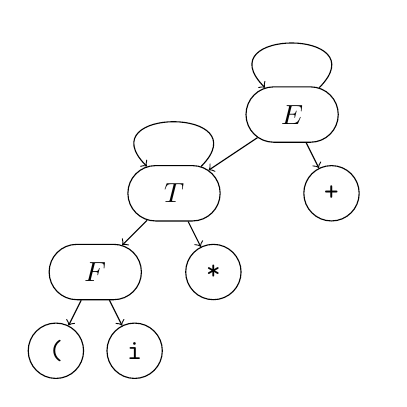
\begin{tikzpicture}
\tikzstyle{mono}=[draw,circle,minimum width=2em,font=\ttfamily];
\tikzstyle{con}=[draw,rounded rectangle,minimum height=2em,minimum width=4em];
\tikzstyle{dir}=[->];
\node [mono] (v2) at (-0.5,1.5) {(};
\node [mono] (v3) at (0.5,1.5) {i};
\node [con] (v1) at (0,2.5) {$F$};
\draw [dir] (v1) edge (v2);
\draw [dir] (v1) edge (v3);
\node [con] (v4) at (1,3.5) {$T$};
\draw [dir] (v4) edge (v1);
\node [mono] (v5) at (1.5,2.5) {*};
\draw [dir] (v4) edge (v5);
\draw [dir] (v4) edge[loop, looseness=4] (v4);
\node [con] (v6) at (2.5,4.5) {$E$};
\draw [dir] (v6) edge (v4);
\draw [dir] (v6) edge[loop, looseness=4] (v6);
\node [mono] (v7) at (3,3.5) {+};
\draw [dir] (v6) edge (v7);
\end{tikzpicture}}
    \subfigure[\textit{LASTVT}依赖关系图]{\usetikzlibrary{shapes}
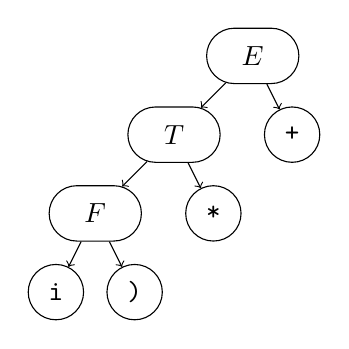
\begin{tikzpicture}
\tikzstyle{mono}=[draw,circle,minimum width=2em,font=\ttfamily];
\tikzstyle{con}=[draw,rounded rectangle,minimum height=2em,minimum width=4em];
\tikzstyle{dir}=[->];
\node [con] (v1) at (-1,0.5) {$E$};
\node [con] (v2) at (-2,-0.5) {$T$};
\node [con] (v3) at (-3,-1.5) {$F$};
\draw [dir] (v1) edge (v2);
\draw [dir] (v2) edge (v3);
\node [mono] (v6) at (-1.5,-1.5) {*};
\node [mono] (v4) at (-3.5,-2.5) {i};
\node [mono] (v5) at (-2.5,-2.5) {)};
\node [mono] (v7) at (-0.5,-0.5) {+};
\draw [dir] (v3) edge (v4);
\draw [dir] (v3) edge (v5);
\draw [dir] (v2) edge (v6);
\draw [dir] (v1) edge (v7);
\end{tikzpicture}}
    \caption{依赖关系图}
\end{figure}

\subsection{三进 DFS}

\paragraph{一进 DFS:归并分类} 现在的依赖关系图依然是有向有环图。根据包含关系的特性,如果出现
\begin{equation*}
    S_1 \subseteq S_2 \subseteq \cdots \subseteq S_n \subseteq S_1
\end{equation*}
所对应的环路
\begin{equation*}
    S_1 \rightarrow S_2 \rightarrow \cdots \rightarrow S_n \rightarrow S_1
\end{equation*}
则这些集合都是相等的:
\begin{equation*}
    S_1 = S_2 = \cdots = S_n
\end{equation*}

使用 DFS 检测环路,并采用类似并查集的方法归并同类的元素,记录每个非终结符所对应的集合号码,以及每一类的非终结符集合。

\begin{table}[h]
    \centering
    \caption{类别号码}\label{tab:num}
    \subfigure[\textit{FIRSTVT}]{
        \begin{tabular}{|c|c|c|}
            \hline
            $F$ & $E$ & $T$ \\
            \hline
            \bfseries 0 &\bfseries 2 &\bfseries 4 \\
            \hline
        \end{tabular}
    }
    \subfigure[\textit{LASTVT}]{
        \begin{tabular}{|c|c|c|}
            \hline
            $F$ & $E$ & $T$ \\
            \hline
            \bfseries 1 &\bfseries 2 &\bfseries 0 \\
            \hline
        \end{tabular}
    }
\end{table}

\paragraph{二进 DFS:连接消环} 通过再一次的 DFS 构造类别之间的 DAG(有向无环图),因为此时同类型内部的环边已经被消除。

\begin{figure}[H]
    \centering
    \subfigure[\textit{FIRSTVT}]{\usetikzlibrary{shapes}
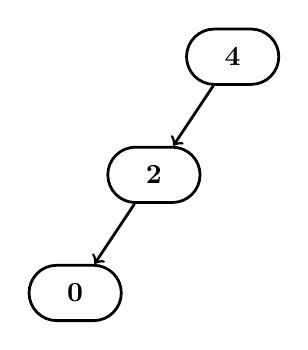
\begin{tikzpicture}[line width=1pt]
\tikzstyle{con}=[draw,font=\bfseries,rounded rectangle,minimum height=2em,minimum width=4em];
\tikzstyle{dir}=[->];

\node [con] (v2) at (-0.5,1) {2};
\node [con] (v3) at (-1.5,-0.5) {0};
\node [con] (v1) at (0.5,2.5) {4};
\draw [dir] (v1) edge (v2);
\draw [dir] (v2) edge (v3);
\end{tikzpicture}}
    \subfigure[\textit{LASTVT}]{\usetikzlibrary{shapes}
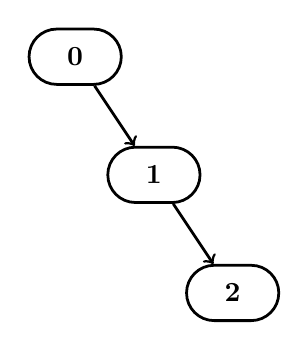
\begin{tikzpicture}[line width=1pt]
\tikzstyle{con}=[draw,font=\bfseries,rounded rectangle,minimum height=2em,minimum width=4em];
\tikzstyle{dir}=[->];

\node [con] (v2) at (1.5,1) {1};
\node [con] (v3) at (2.5,-0.5) {2};
\node [con] (v1) at (0.5,2.5) {0};
\draw [dir] (v1) edge (v2);
\draw [dir] (v2) edge (v3);
\end{tikzpicture}}
    \caption{类别连接}\label{fig:conn}
\end{figure}

\paragraph{三进 DFS:映射输出} 对于每一个非终结符,查类别号码表 \ref{tab:num} 得到其对应类别,然后在类别连接图 \ref{fig:conn} 中从该类别节点进行 DFS,合并路上对应的终结符节点,就可以得到该非终结符对应的集合。

\begin{table}[h]
    \centering
    \caption{集合}
    \subfigure[\textit{FIRSTVT}]{
        \begin{tabular}{c|>{\ttfamily}l}
            \hline
            $E$ & i + ( * \\
            \hline
            $T$ & i ( * \\
            \hline
            $F$ & i ( \\
            \hline
        \end{tabular}
    }
    \subfigure[\textit{LASTVT}]{
        \begin{tabular}{c|>{\ttfamily}l}
            \hline
            $E$ & i + ) * \\
            \hline
            $T$ & i ) * \\
            \hline
            $F$ & i ) \\
            \hline
        \end{tabular}
    }
\end{table}

\subsection{识别关系}

最后一步,就是根据定义 \ref{def:opn} 来遍历产生式检测终结符号之间的优先关系了。在识别之前,需要现在产生式的集合中加入对于开始符号的输入首尾标记:
\begin{equation*}
    E \rightarrow \$ E \$
\end{equation*}
因为该符号比较特殊,其优先级是额外定义的\cite{opgwiki}:
\begin{equation*}
    \$ < T, T > \$, \$=\$,\quad \forall T\in V_T
\end{equation*}
并不属于原有的语法,所以要在这个地方再加入。

最终就可以得到本部分开头的程序输出。

\section{函数接口}

以下是运行样例 1 时由 uftrace\cite{uft} 生成的函数调用列表。
% 接口调用
\lstinputlisting[language=c,basicstyle=\scriptsize\ttfamily, commentstyle=\color{green!50!black}]{img/replay.txt}

% uftrace 跟踪函数调用
\begin{figure}[H]
    \centering
    % \rotatebox{90}{
        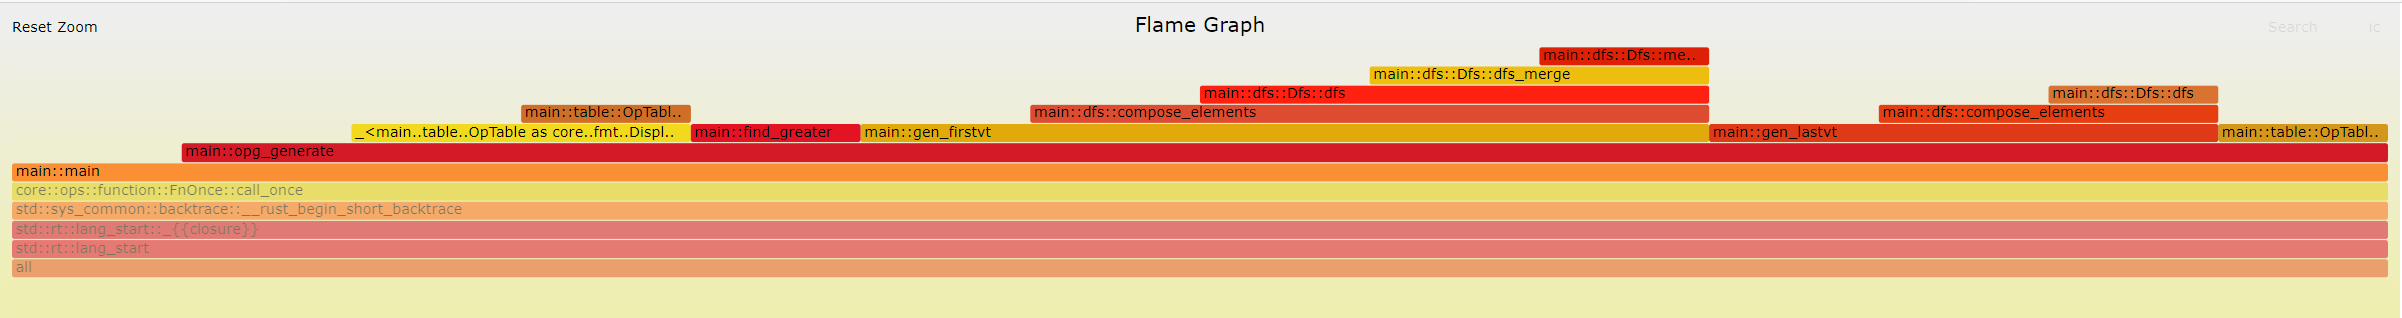
\includegraphics[width=\textwidth]{img/flame.png}
    % }
    \caption{火焰图\cite{flame}}
    \label{fig:flame}
\end{figure}

以上结果由 \href{run:../opg/uftrace.sh}{该脚本} 生成。关于函数的更多信息,请访问 \href{run:../opg/target/doc/opg/index.html}{API 文档}。% 使用 cargo doc 编译。

\part{卷积优化}
\subsection*{运行截图}
\begin{figure}[H]
    \centering
    \subfigure[raw1]{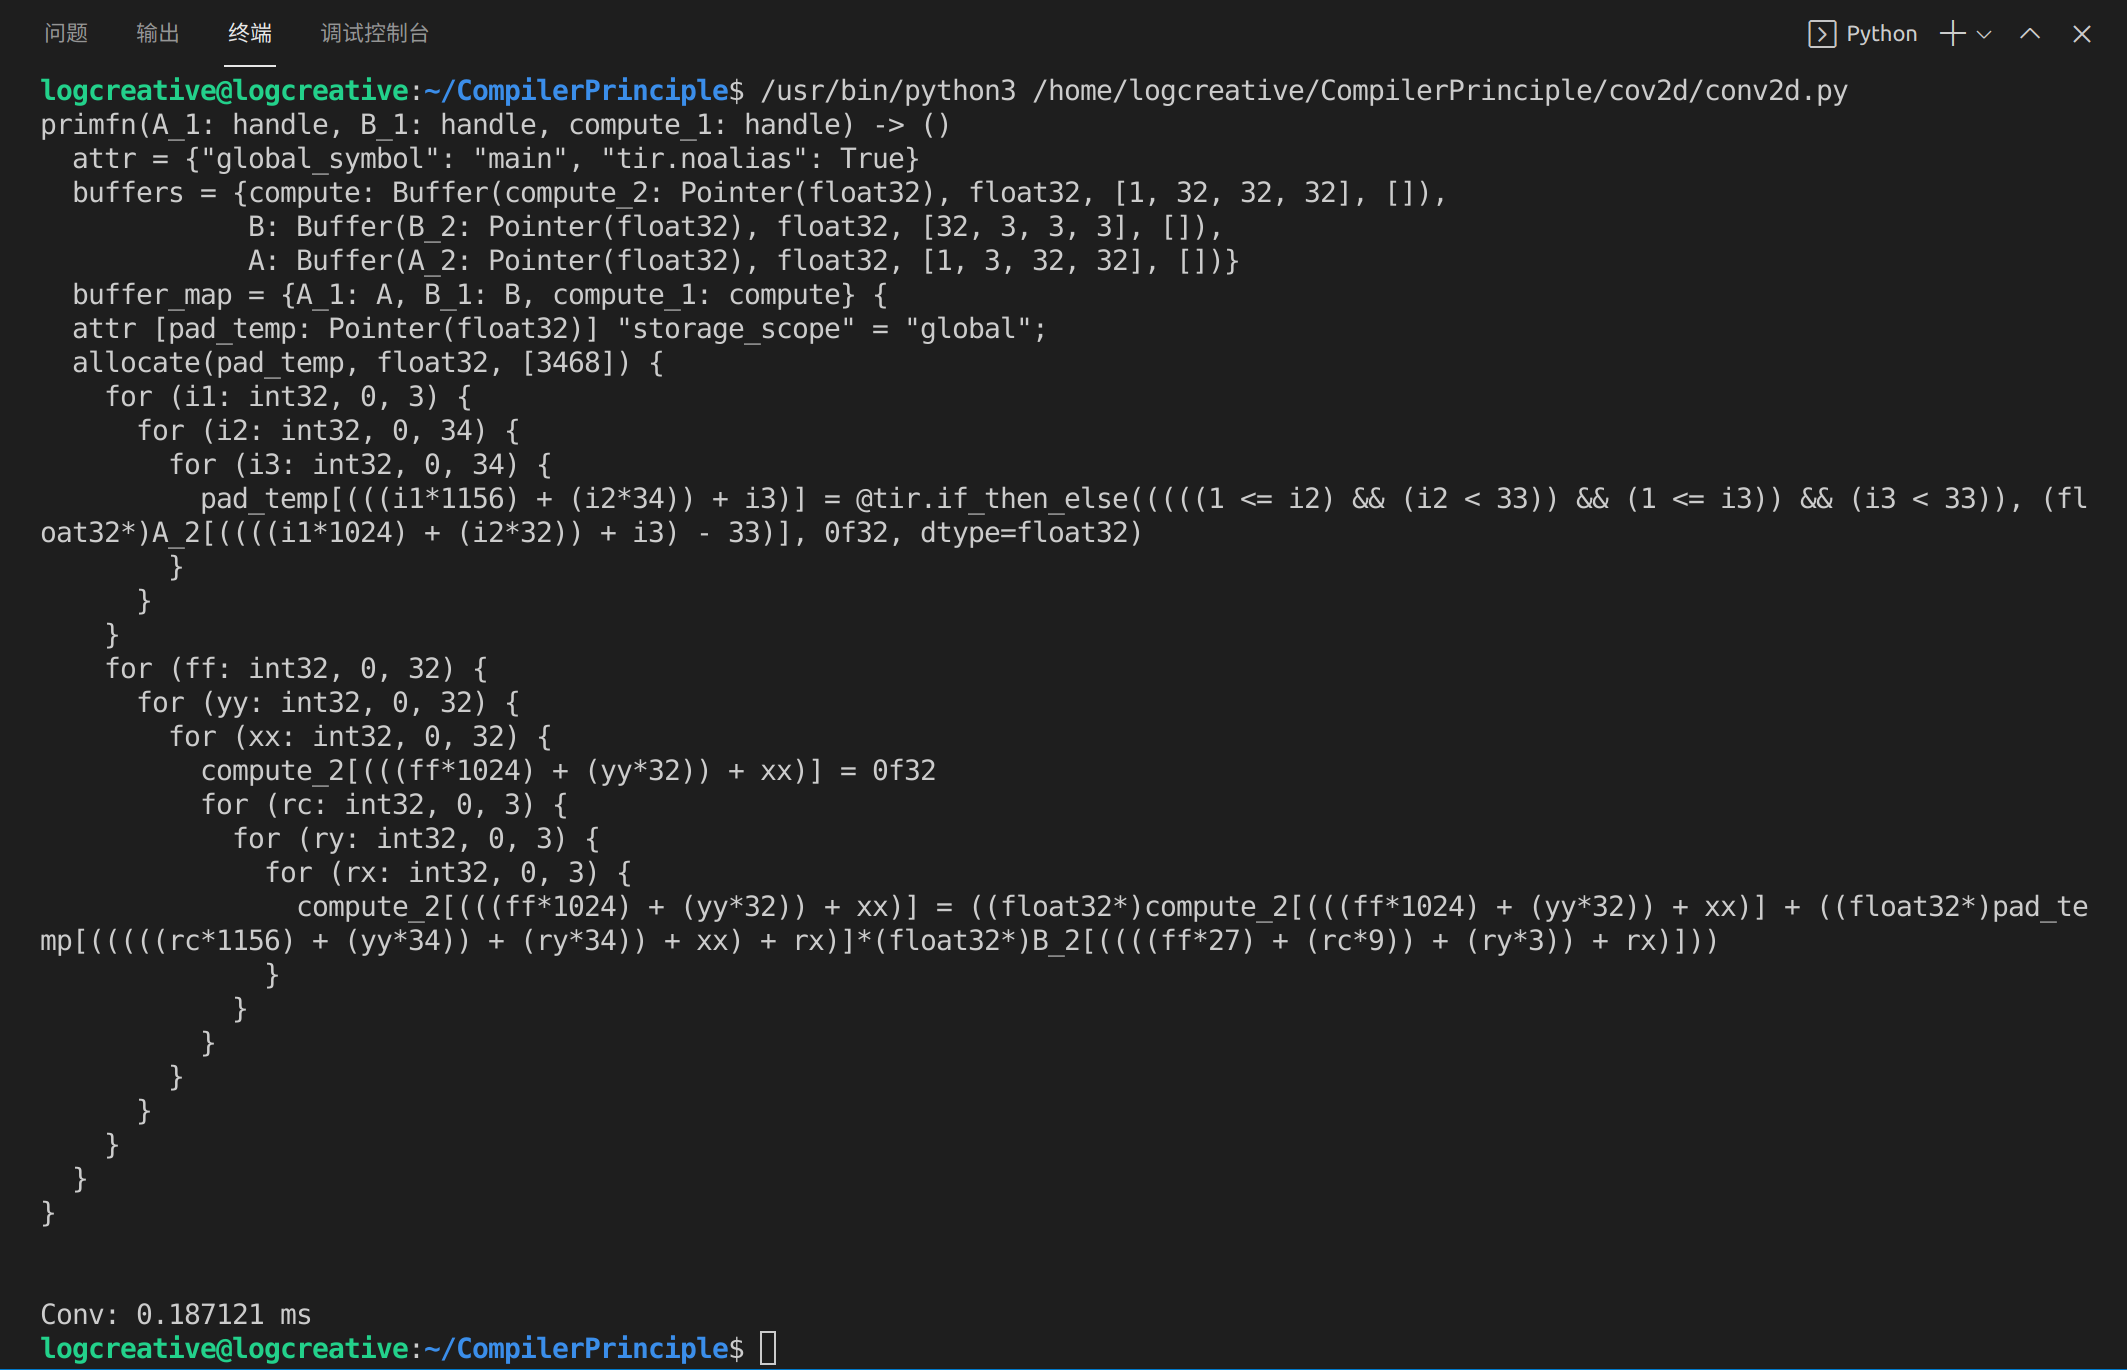
\includegraphics[width=0.45\textwidth]{img/raw1.png}}
    \subfigure[op1]{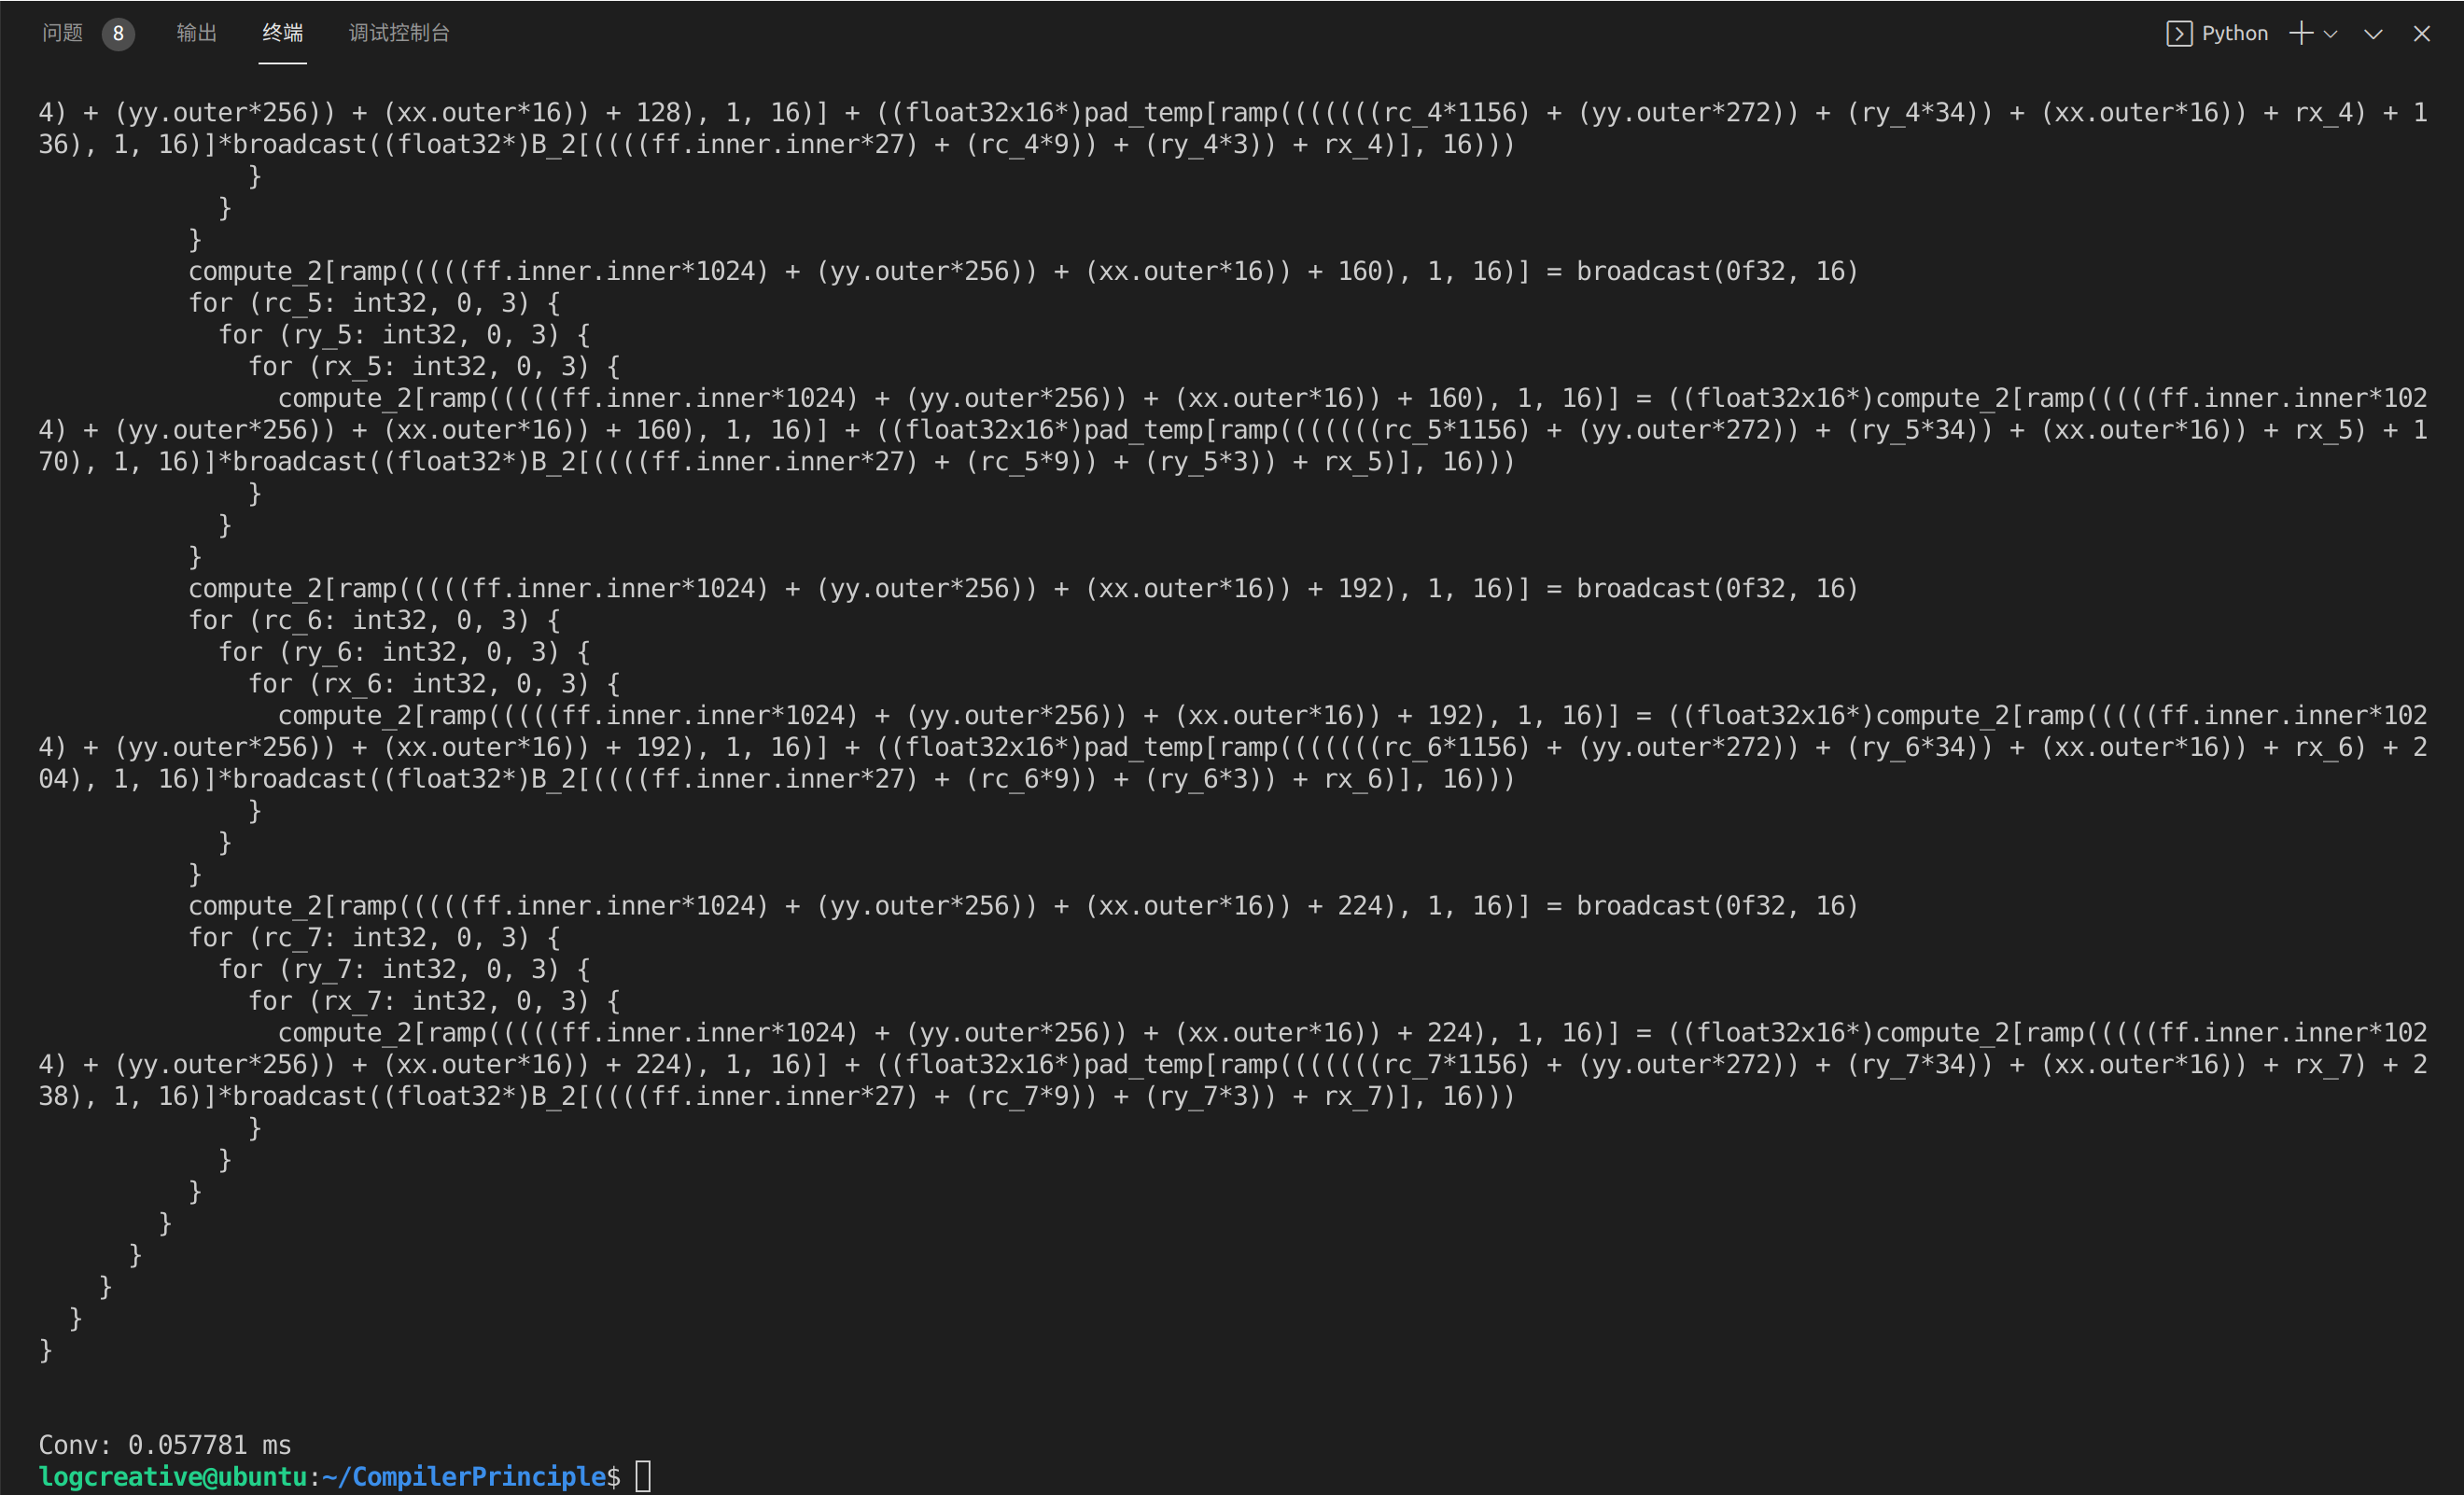
\includegraphics[width=0.45\textwidth]{img/op1.png}}
    \subfigure[raw2]{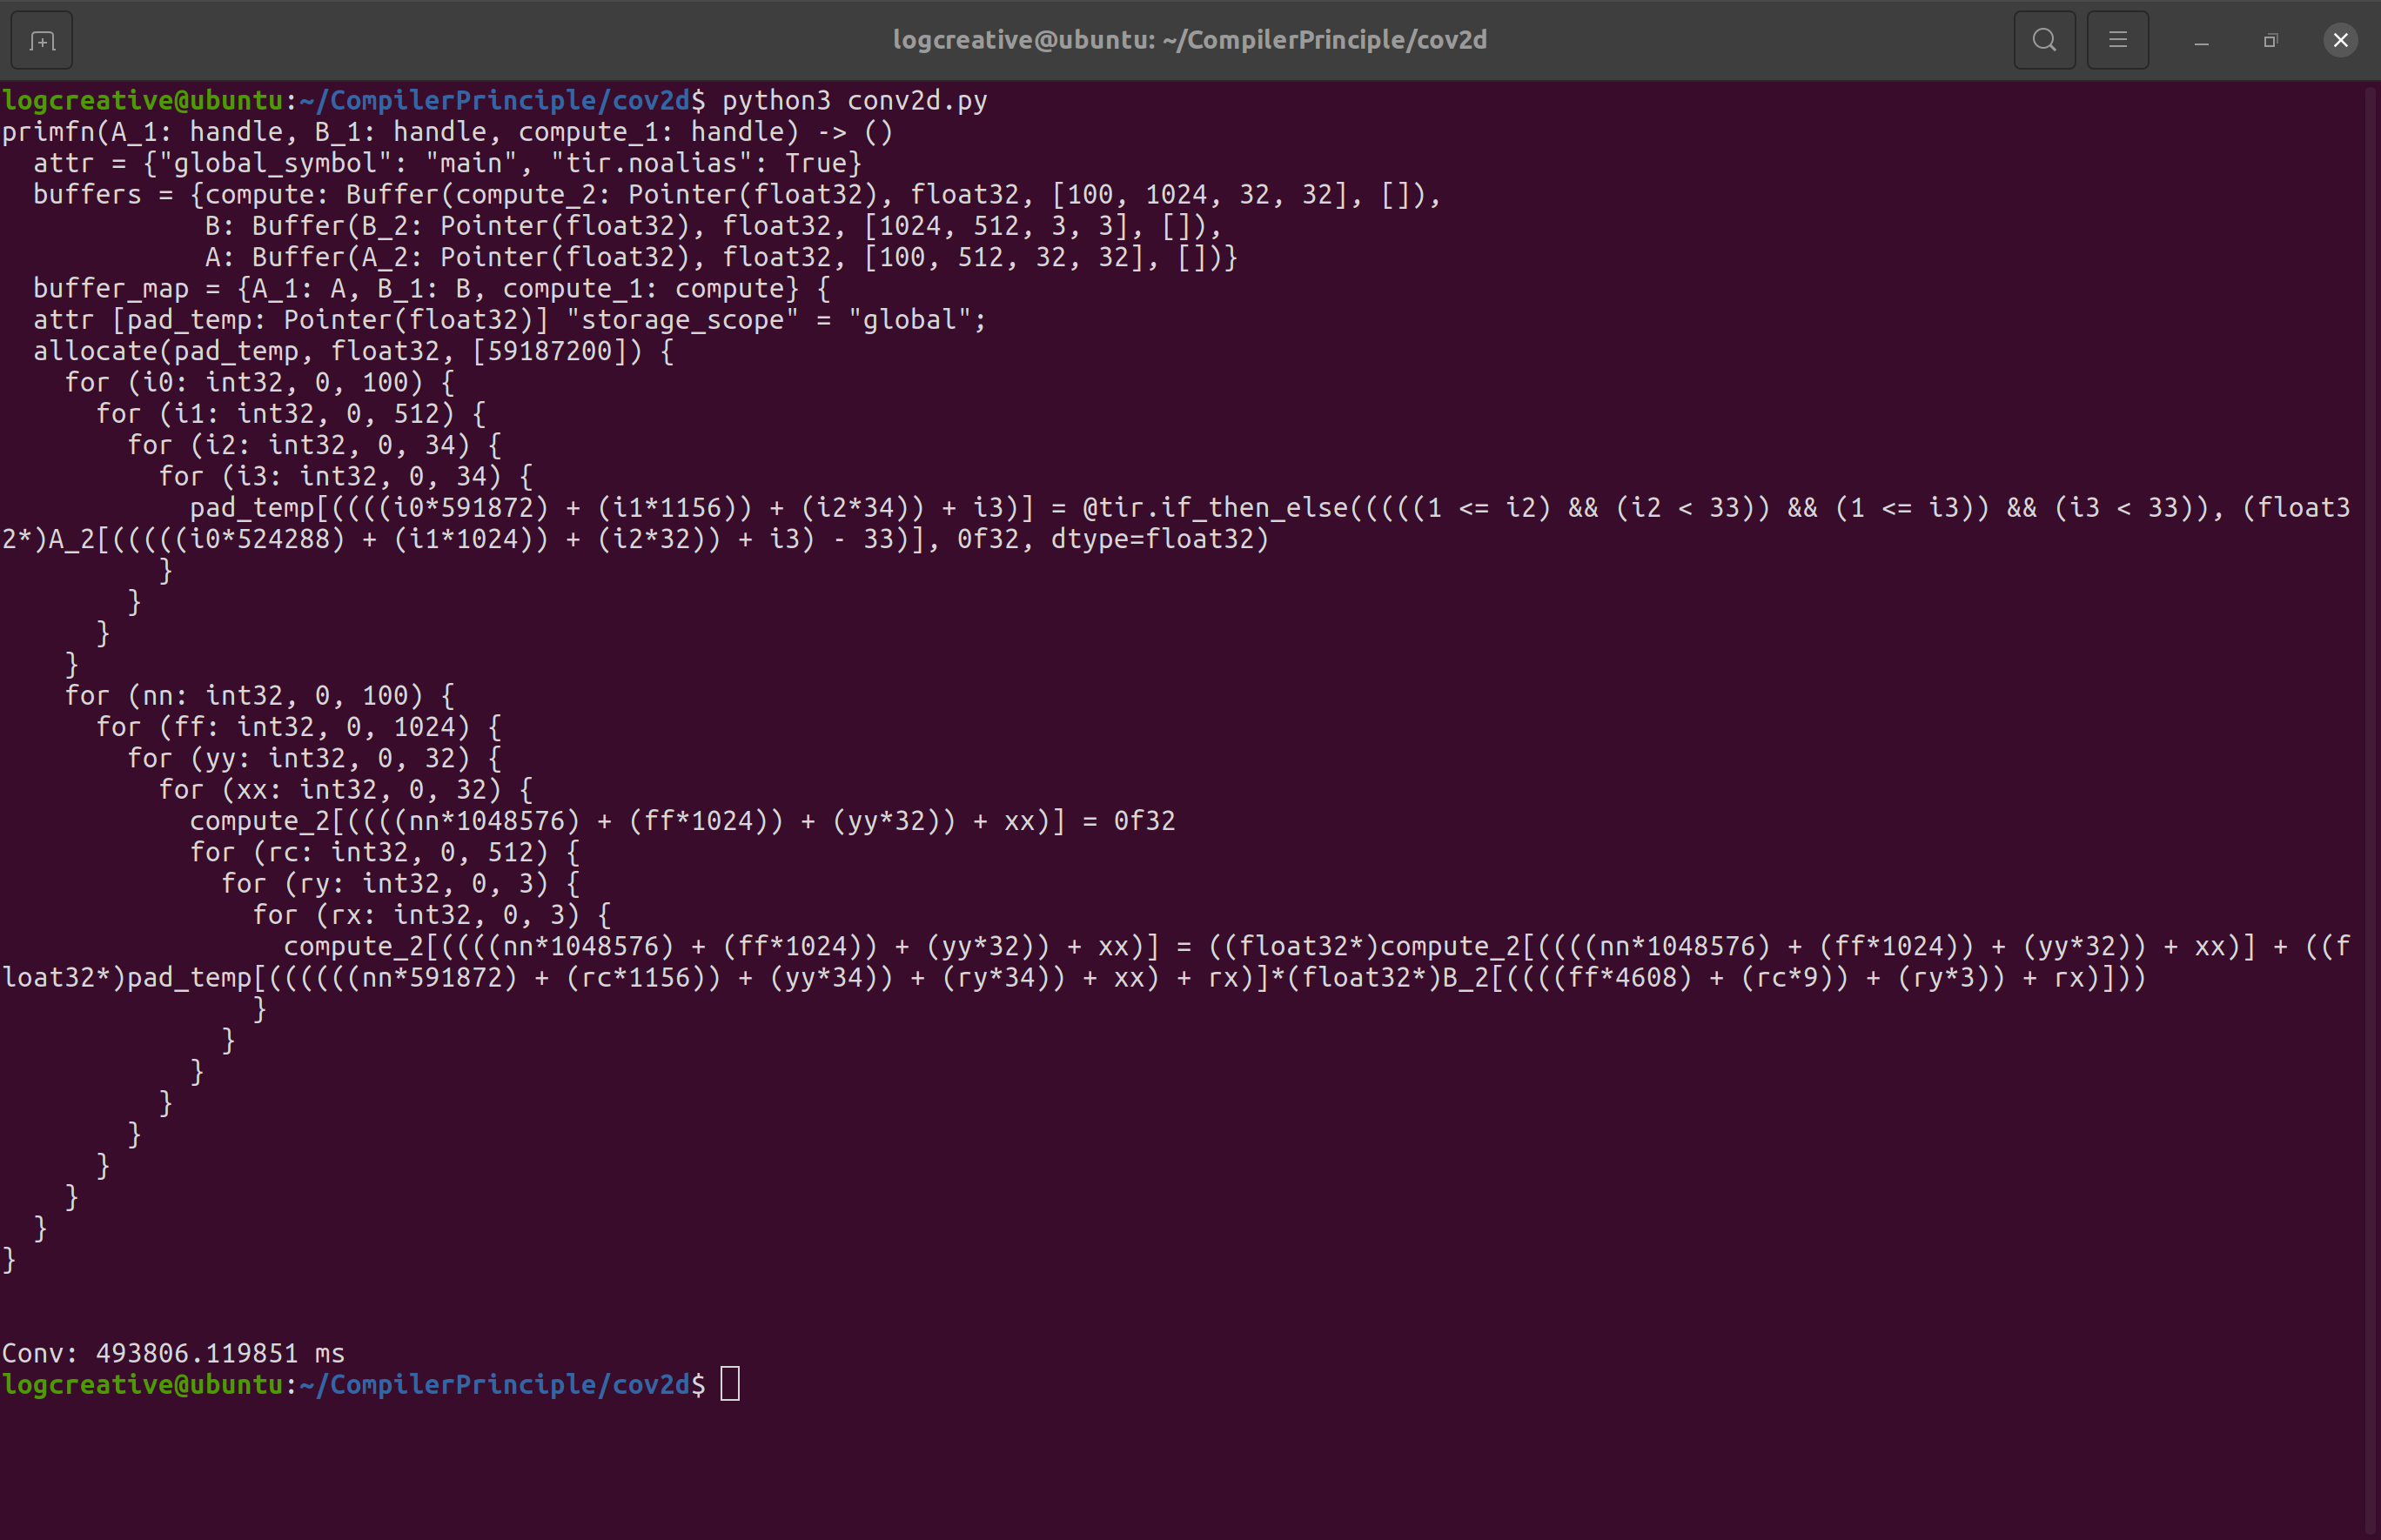
\includegraphics[width=0.45\textwidth]{img/raw2.png}}
    \subfigure[op2]{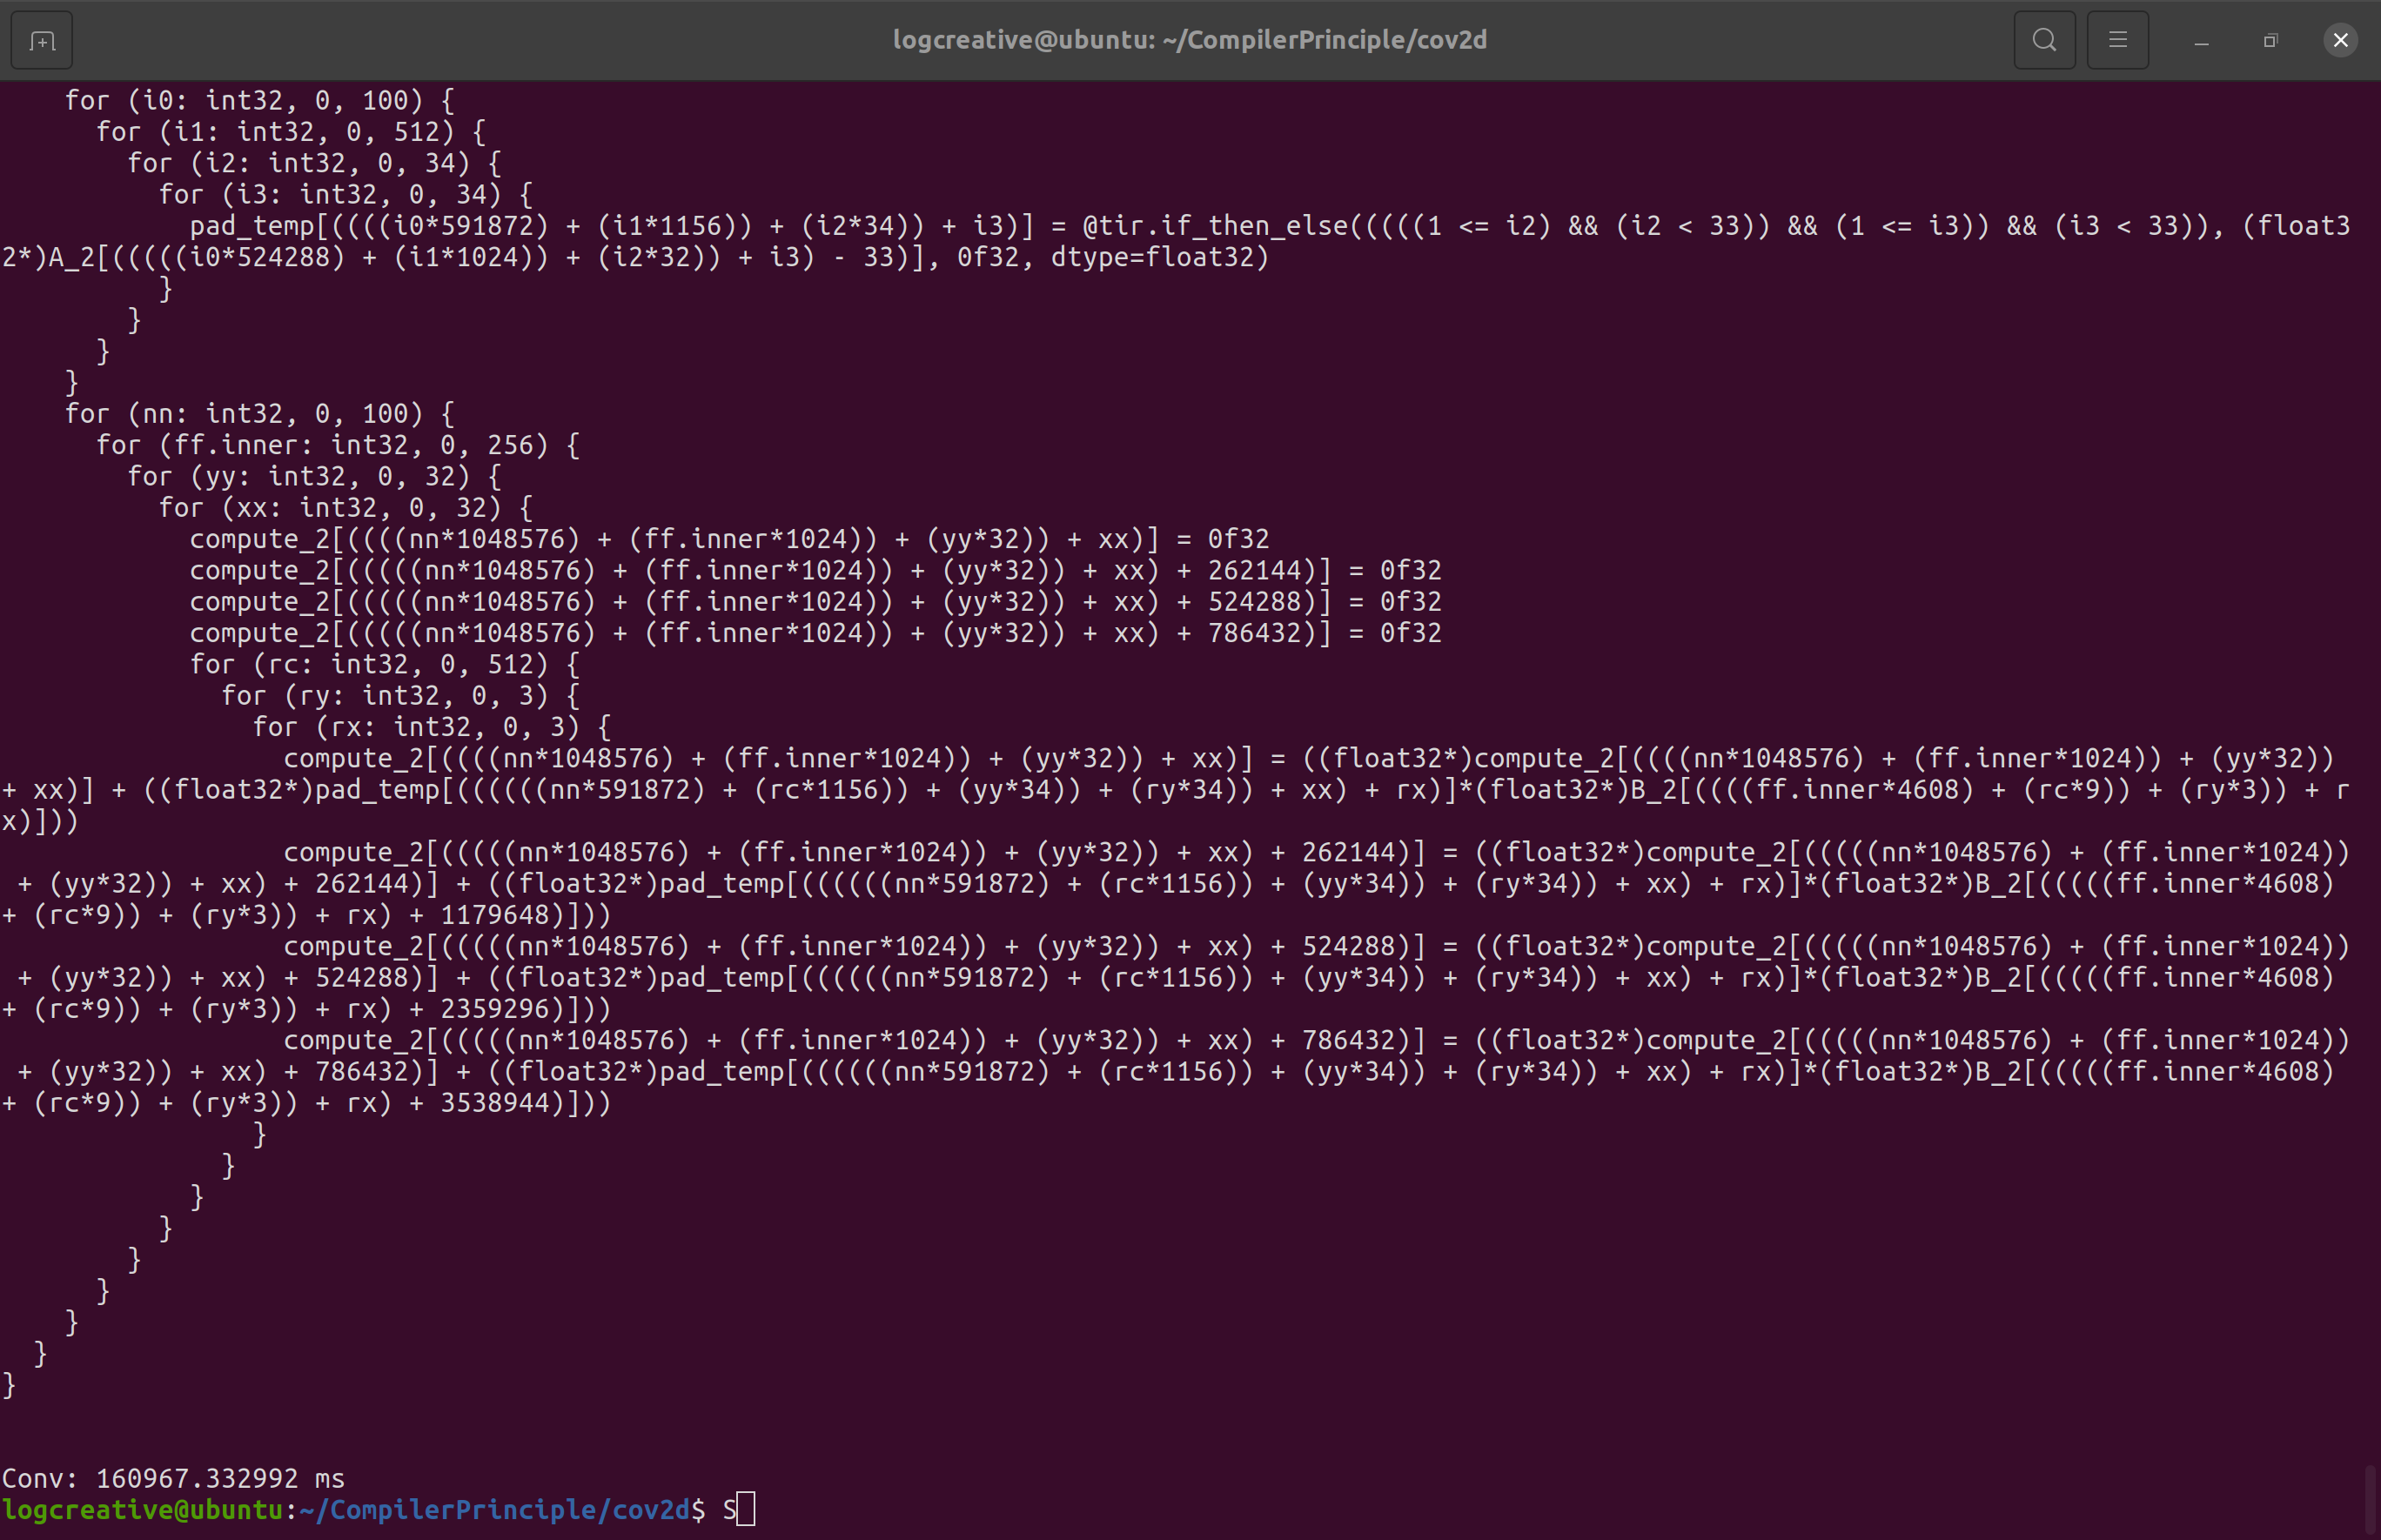
\includegraphics[width=0.45\textwidth]{img/op2.png}}
\end{figure}

\subsection*{优化结果}
\begin{table}[H]
    \begin{tabular}{m{17em}rrc}
        \toprule
        输入大小和输出大小 & 优化前 & 优化后 & 提升效率 \\
        \midrule
        \ttfamily
        n, ic, ih, iw = 1, 3, 32, 32~~~~~
        oc, kh, kw = 32, 3, 3
        & 0.165312 ms & 0.057781 ms & 65.0\%\\
        \hline
        \ttfamily
        n, ic, ih, iw = 100, 512, 32, 32
        oc, kh, kw = 1024, 3, 3
        & 493806.119851 ms & 160967.332992 ms & 67.4\%\\
        \bottomrule
    \end{tabular}
\end{table}

% raw 2-1: 493806.119851 ms
% raw 2-2: 496377.535468 ms

% Virtual Multithreading for large matrix

\bibliography{ref}

\end{document}
